\title{Změny skupenství}
\documentclass[10pt,a4paper]{article}
\usepackage[utf8]{inputenc}
\usepackage[czech]{babel}
\usepackage{amsmath}
\usepackage{amsfonts}
\usepackage{amssymb}
\usepackage{chemfig}
\usepackage{geometry}
\usepackage{wrapfig}
\usepackage{graphicx}
\usepackage{floatflt}
\usepackage{hyperref}
\usepackage{fancyhdr}
\usepackage{tabularx}
\usepackage{makecell}
\usepackage{csquotes}
\usepackage{footnote}
\usepackage{movie15}
\MakeOuterQuote{"}

\renewcommand{\labelitemii}{$\circ$}
\renewcommand{\labelitemiii}{--}
\newcommand{\ra}{$\rightarrow$ }
\newcommand{\x}{$\times$ }
\newcommand{\lp}[2]{#1 -- #2}
\newcommand{\timeline}{\input{timeline}}


\geometry{lmargin = 0.8in, rmargin = 0.8in, tmargin = 0.8in, bmargin = 0.8in}
\date{\today}
\author{Jakub Rádl}

\makeatletter
\let\thetitle\@title
\let\theauthor\@author
\makeatother

\hypersetup{
colorlinks=true,
linkcolor=black,
urlcolor=cyan,
}



\begin{document}
\maketitle
\tableofcontents
\begin{figure}[b]
Toto dílo \textit{\thetitle} podléhá licenci Creative Commons \href{https://creativecommons.org/licenses/by-nc/4.0/}{CC BY-NC 4.0}.\\ (creativecommons.org/licenses/by-nc/4.0/)
\end{figure}
\newpage

\paragraph{Otázečky}
\begin{enumerate}
\item Které skupenství převládá v SS? [plazma]
\item Proč nás větrák ochlazuje? [ochlazování odpařováním (vítr odnáší vlhký vzduch)]
\item Jak vzniká déšť, mlha, rosa? []
\item Jaké počasí očekávat při přechodu teplé fronty?
\item Co je trojný bod?
\end{enumerate}

\section{Změny skupenství}
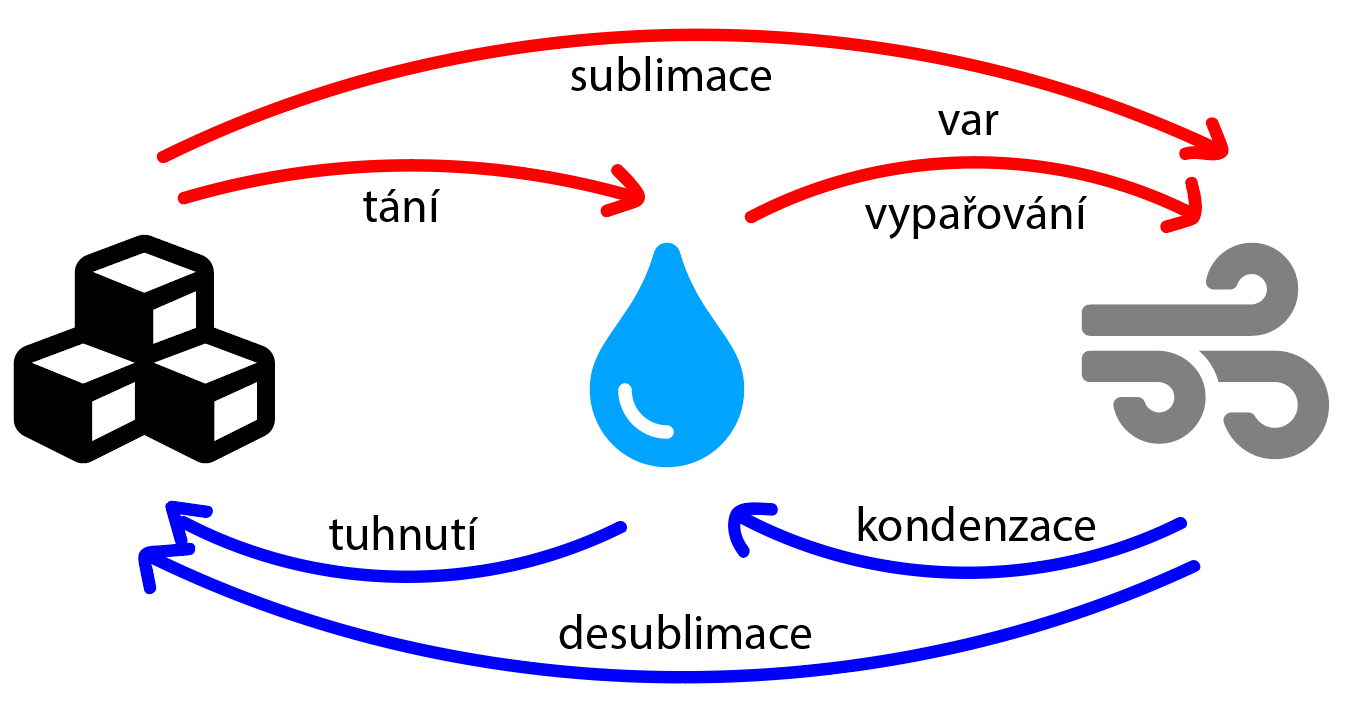
\includegraphics[width=1\textwidth]{pictures/premena_skupenstvi.png}
\begin{itemize}
\item změny v mikrostruktuře, vazbách látky
\end{itemize}

\paragraph{Skupenské teplo}
$$L_t = m \cdot l_t$$
\begin{itemize}
\item $L_t$ \ldots skupenské teplo potřebná k roztání látky [J]
\item $l_t$ \ldots měrné skupenské teplo [J/kg]
\end{itemize}

\paragraph{Př.:} kolik tepla je potřeba k ohřátí kilogramu ledu(-10) na 20 stupňovou vodu?
\begin{itemize}
\item $C_l = 2.1$ kJ/kg/K
\item $C_v = 4.2$ kJ/jg/K
\item $l_t = 334$ kJ/kg
\item $Q_1 = mc_l\Delta T = 1*2100*10 = 21$kJ
\item $Q_2 = ml_t = 1*334000 = 334$kJ
\item $Q_3 = mc_v\Delta T = 1*4200*20 = 84$kJ
\item $Q = Q_1 + Q_2 + Q_3 = 439$kJ
\end{itemize}

\paragraph{Př.:}

\paragraph{Fázový diagram}
\begin{itemize}
\item závsilost tlaku na teplotě
\end{itemize}

\subsection{Tání a tuhnutí}
\begin{itemize}
\item \textbf{krystalizační jádra} -- vznikají okolo nich krystaly při tuhnutí
\item \textbf{přechlazená kapalina} -- $t < t_T$
	\begin{itemize}
	\item mrznoucí déšť
	\end{itemize}
\item svařování -- roztavení, spojení, utuhnutí
\item rtuť -- $t_T = -30^\circ$C
\item wolfram -- $t_T \doteq 3400^\circ$C
\end{itemize}

\subsection{Vypařování a kondenzace}
\begin{itemize}
\item \textbf{vypařování} -- probíhá na povrchu
	\begin{itemize}
	\item závisí na tlaku par nad kapalinou
	\end{itemize}
\item \textbf{var} -- probíhá v celém objemu
	\begin{itemize}
	\item teplotu varu určíme z fázového diagramu
	\end{itemize}
\item \textbf{kondenzace} -- důležitá přítomnost \textbf{kondenzačních jader}
\item \textbf{destilace} -- metoda separace látek na základě rozdílné teploty varu
\end{itemize}

\section{Pracovní list}
\paragraph{Úloha 8}
\begin{itemize}
\item[a)] roztavení \ra propojení \ra zatuhnutí
\item[b)] povrchové tání
\item[c)] v dešti
\item[d)] ve skleníku, kuchyni bez digestoře nebo v pralese
\item[e)] oteplení studeného vzduchu z venku 
\item[f)] nefunguje pocení
\item[g)] nízká maximální vlhkost \ra rychlejší kondenzace
\item[h)] separace látek na základě různé teploty varu
\item[i)] tlakem zvyšuje teplotu varu vody \ra připravování potravin při vyšší teplotě
\item[j)] 
\end{itemize}


\end{document}